\subsection{Data Processing}


% \renewcommand{\arraystretch}{1.2}
% \begin{table*}[ht]
% \small
% \centering
% \begin{tabular}{|p{4.2cm} | p{3.7cm} | p{3.8cm} | p{3.4cm}|} \hline
% \multicolumn{2}{|c|}{\textbf{Physiological Measures}} & \multicolumn{2}{|c|}{\textbf{Performance Measures}} \\ \hline 
% \multicolumn{1}{|c|}{Raw} & \multicolumn{1}{|c|}{Derivative} & \multicolumn{1}{|c|}{Primary Task} & \multicolumn{1}{|c|}{Secondary Task} \\ \hline
% Electrocardiogram (ECG) & Pulse Transit Time (PTT) & Steering Deviation & Sentence Response Time \\ 
% Photoplethysmograph (PPG) & Inst. Heart Rate (IHR)} & Acceleration Reaction Time & Sentence Accuracy \\ 
% Impedance Cardiography(ICG) & SKT B $-$ SKT A (SKT) & Acceleration Accuracy & Math Response Time \\ 
% Respiration  & & Braking Reaction Time & Math Accuracy  \\ 
% Electrodermal Activity (EDA)  & &  Braking Accuracy & Recall Accuracy \\ 
% Skin Temp. Nose (SKT A) & &  & \\ 
% Skin Temp. Cheek (SKT B) & &  & \\ 
% Electromyography (EMG) & &  & \\ 
% Pupil Dilation  & &  & \\ 
% Eye Gaze &  &  & \\
% \hline\end{tabular}
% \caption{Collection of measures available in the dataset.}
% \label{table:measures}
% \end{table*}

\renewcommand{\arraystretch}{1.1}
\begin{table*}[ht]
\small
\centering
\begin{tabular} {@{}llcll@{}}\toprule
\multicolumn{2}{c}{\textbf{Physiological Measures}} &  \phantom{abc} & \multicolumn{2}{c}{\textbf{Performance Measures}} \\ 
\cmidrule{1-2} \cmidrule{4-5}
\multicolumn{1}{c}{Raw} & \multicolumn{1}{c}{Derivative} && \multicolumn{1}{c}{Primary Task} & \multicolumn{1}{c}{Secondary Task} \\ \midrule
Electrocardiogram (ECG) & Pulse Transit Time (PTT) && Steering Deviation & Sentence Response Time \\ 
Photoplethysmograph (PPG) & Inst. Heart Rate (IHR) && Acceleration Reaction Time & Sentence Accuracy \\ 
Impedance Cardiography(ICG) & SKT B $-$ SKT A (SKT) && Acceleration Accuracy & Math Response Time \\ 
Respiration  & && Braking Reaction Time & Math Accuracy  \\ 
Electrodermal Activity (EDA)  & &&  Braking Accuracy & Recall Accuracy \\ 
Skin Temp. Nose (SKT A) & &&  & \\ 
Skin Temp. Cheek (SKT B) & &&  & \\ 
Electromyography (EMG) & &&  & \\ 
Pupil Dilation  & &&  & \\ 
Eye Gaze &  &&  & \\
\bottomrule
\end{tabular}
\caption{Collection of measures available in the dataset.}
\label{table:measures}
\end{table*}


\begin{figure*}[th]
\centering
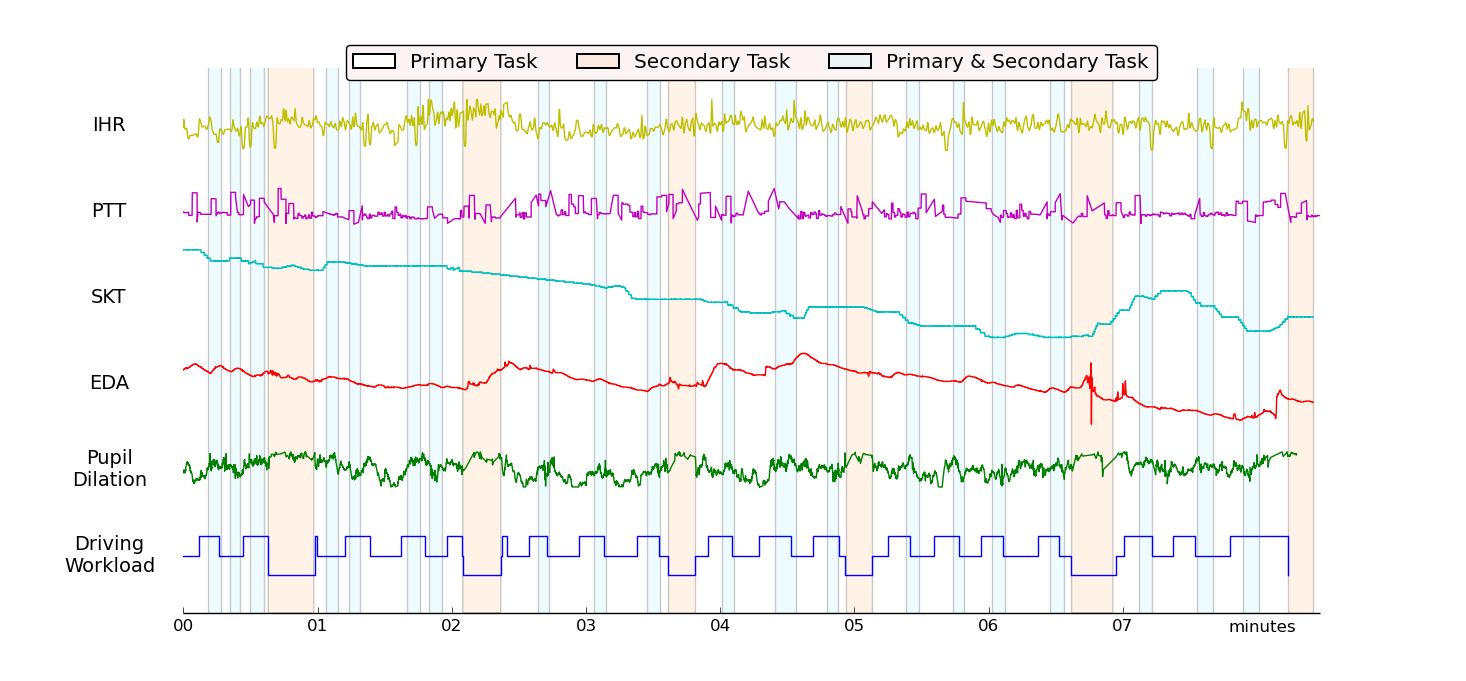
\includegraphics[height=8cm]{bwrepr}
\vspace{-1.5em}
\caption{Example physiological measures collected during an audio non-mediated experimental condition. Driving workload is represented as a step function (1: High, 0: Low, -1: Pause). Shaded regions delineate when the user was engaged in the primary driving task (P),  secondary notification task (S), or both (P \& S).}
\label{fig:snapshot}
\end{figure*}

The dataset consists of a number of physiological and performance measures which are tabulated in Table~\ref{table:measures}. We recorded ten psychophysiological signals: EDA, EMG, Skin temperatures (nose \& cheek), four signals based on cardiac activity (ECG, PPG, ICG \& Respiration), and two based on eye activity (gaze \& pupil dilation). Apart from the eye-based signals, which were sampled at 30 Hz, the rest of the signals were sampled at 2000 Hz. 

Three derivative signals were also calculated. Instantaneous heart rate (IHR) was obtained from the ECG signal using the BioSig library\footnote{http://biosig.sourceforge.net/} which implements Berger's algorithm~\cite{berger1986}). Pulse Transit Time (PTT) was obtained by calculating the difference in between the ECG R-wave peak time and the PPG peak time, which is the time it takes for the pulse pressure waveform to propagate through a length of the arterial tree. Difference in skin temperature (SKT) was also calculated by subtracting the temperature of the nose from that of the cheek.

The performance measures encompass both the primary driving task and the secondary notification task. Of interest are the reaction times and accuracies to the red and green light stimuli, and the steering deviation in tracking the reference cylinder. Also recorded are the performance measures for the secondary notification task as shown in Table~\ref{table:measures}.

\subsubsection{Preprocessing \& Labelling}
We analyzed the following five physiological signals: IHR, PTT, SKT, EDA and Pupil Dilation (Figure~\ref{fig:snapshot}). These signals were extracted from the rosbags and down-sampled to 40 Hz (except for pupil which remains at its original sampling rate of 30 Hz). Each signal was plotted, and thresholds were determined to filter out unlikely values (from movement artifacts, etc.). Data for each user was standardized (zero mean \& unit variance), prior to which outliers that were greater than three standard deviations were filtered out.

Two sets of labels are included in the dataset, one each for the primary and secondary task. By syncing with the timestamps from both the task logs, we determined the precise primary and secondary task conditions that the participant was under for every physiological sample. The primary task labels denotes if the participant is in the low, high or paused driving workload condition (see Driving Workload in Figure~\ref{fig:snapshot}). The logs from the secondary task allow us to determine the periods during which a participant was attending to a notification, i.e.\ blue regions in Figure~\ref{fig:snapshot}. The orange regions signify the recall part of the secondary task, when the primary driving task was paused.

\subsection{Feature Extraction}
We derived a number of statistical features on the main signal (x[n]), the derivative signal $(x[n+1] - x[n])$, and the percentage change $((x[n+1] - x[n])/x[n] * 100)$. These features include the mean, median, percentiles (\nth{10}, \nth{25}, \nth{75}, \nth{90}), ranges (between min and max, \nth{10} and \nth{90} percentiles, and \nth{25} and \nth{75} percentiles), skewness, standard deviation.

Features were extracted by moving a convolving data (3 to 7 datum) window across the signal. To capture some of the temporal properties, windows were overlapped by setting the step size to be smaller than the window size. Different window and step size lengths were considered. Specifically, the following pairs of window and step sizes (seconds) were analyzed: (7, 1), (5, 1), (3, 1) and (3, 0.25). 

\subsection{Modelling for Multitasking Scenario}
Based on the insights from Wilkin's multiple resource theory described in the section 2.2,  the primary and secondary tasks should no be not mutually exclusive, since resources along particular dimensions are shared. Thus, we can view this as a multilabel classification problem. In this formulation, each window is assigned two labels to denote the two possible tasks that the participant can be engaged in, for the duration of that window. For the purposes of this evaluation, the specific states of both tasks (low/high; attending/recall) are ignored reducing this to a multilabel binary classification problem. 

For the duration of the window, if the participant is only engaged in the primary driving task, the window is labelled as P. If the driving task is paused, and the participant is engaged in recall, the window is labelled as S. Since the duration of attending to a notification is usually shorter than 7 seconds, windows where a participant is attending to a notification for at least the first half while driving for the whole duration are labelled as both P and S. All other transitory windows were discarded.   

The features for each window, and the corresponding multilabel assigments \{P,S\} were fed to a Random Forest classifier, which is an ensemble technique that learns a number of decision tree classifiers and aggregates their results. Models were built across all users, as well as for each user separately, so as to account for individual differences in their psychophysiological response. To evaluate the classifier's performance, we used leave-one-user-out cross-validation for the population models, and 3-fold cross-validation for the individual user models. 

The time it takes to comprehend a notification varies by participant. This creates variation in the number of driving and notification task labels generated per participant, which in turn results in a varying baseline accuracy for each user. Hence, we report the area under  the Receiver Operating Characteristic (ROC) curve (AUC) instead of accuracy. ROC curves show the tradeoffs between higher sensitivity and higher specificity. Sensitivity refers to the correct detection of a condition or state when it is truly present. Specificity indicates the correct rejection of a state when it is truly not present. The area under the ROC curve is a measure of adequacy on both. Curves corresponding to random or chance classification of 50\% would fall close to the diagonal, and result in an ROC AUC score of 0.5, while the most successful classifications would have an ROC AUC score close to 1.0. 

Being a multilabel classification problem, the classifier outputs two probabilities simultaneously: one for the probability of the sample belonging to the primary task (P), and another for the probability that the sample belongs to the secondary task (S). We report the macro-averaged ROC AUC scores for the pair of labels, as a measure of how well the classifier is able to predict both labels (P, S). We also report the ROC AUC score for each label, individually, to shed light on how accurately the classifier is able to identify each task.

\subsection{Results}

\renewcommand{\arraystretch}{1.2}
\begin{table}[t]
\centering
\begin{tabular} {@{}ccrrrcrrr@{}}\toprule
\multirow{2}{*}{\parbox[c]{1.3cm}{\centering Window,\\Step (s)}} & \phantom{}
&  \multicolumn{3}{c}{Population} & \phantom{} & \multicolumn{3}{c}{Individual} \\
\cmidrule{3-5} \cmidrule{7-9}
%  && \multicolumn{1}{c}{P, S} & \multicolumn{1}{c}{P} & \multicolumn{1}{c}{S} && \multicolumn{1}{c}{P, S}& \multicolumn{1}{c}{P} & \multicolumn{1}{c}{S} \\
 && P, S & P & S && P, S & P & S\\
\midrule
7, 1 && 0.85 & 0.90 & 0.80 && 0.84 & 0.89 & 0.78 \\
5, 1 && 0.84 & 0.89 & 0.78 && 0.83 & 0.88 & 0.78 \\
3, 1 && 0.81 & 0.85 & 0.76 && 0.81 & 0.87 & 0.75 \\
3, 0.25 && 0.80 & 0.86 & 0.75 && 0.80 & 0.86 & 0.74 \\
\bottomrule
\end{tabular}
\caption{ROC AUC Scores for population and individual models using different window and step sizes}
\label{Tab:win}
\end{table}

For the four window and step size combinations considered, mean ROC AUC scores for the population and individual models are shown in Table~\ref{Tab:win}. A larger window size tends to provide better results, and this trend holds for both the individual and population models. The population scores are comparable to the average user scores, which tells us that the model based on pupil dilations is generalisable. 

Table~\ref{Tab:win} also shows ROC AUC scores for predicting each label individually. The scores indicate that the models are better at identifying when the user is engaged in the primary driving task (P) as compared to when the user is engaged in the secondary notification task (S). This might be because of the differences in load induced by equation and sentence notifications, and also from the differences in the notifications being right or wrong. Our model doesn't account for these yet, but each can be treated as a different class under the multilabel multiclass framework.


\begin{table}
\centering
\begin{tabular}{@{}rcrrr@{}}\toprule
Condition & \phantom{abc} & P, S & P & S\\
 \midrule
\multicolumn{1}{l}{\textit{Non-mediated \phantom{abcde}}} \\
 Video  && 0.88 & 0.90 & 0.86 \\
 Audio  && 0.90 & 0.92 & 0.88 \\
 Overall && 0.88 & 0.91 & 0.86 \\
\multicolumn{1}{l}{\textit{Mediated}} \\
 Video && 0.82 & 0.89 & 0.76 \\
 Audio && 0.81 & 0.88 & 0.74 \\
Overall && 0.81 & 0.89 & 0.74 \\
 \bottomrule
\end{tabular}
\caption{Population-based ROC AUC Scores under different timing and modality conditions.}
\label{Tab:NM}
\end{table}

We also compared how varying the independent variables of timing and modality impacted the ROC AUC scores. The results for these experiments are tabulated in Table~\ref{Tab:NM}. Only the analysis on the 7 second long windows are presented here as similar trends were observed for the other combinations. It is clear that mediating when notifications were sent, had a larger effect than modality, on the model's ability to identify the secondary task. To explain this, we must remember that in the mediated condition, the participant is sent notifications when they are in the low driving-workload state. Te multiple resource theory, projects that  the cognitive load on the user in this state is similar to the cognitive load they experience when they are in the high driving-workload state. Thus, there is an overlap between windows with and without the S label. In the non-mediated condition, this overlap is much smaller, as notifications are also delivered in the high driving-workload states. This allows the classifier to better identify the secondary task in the non-mediated condition.






